\documentclass[letter]{article}

\usepackage[english]{babel}
\usepackage[utf8]{inputenc}
\usepackage{amsmath}
\usepackage[colorinlistoftodos]{todonotes}
\usepackage{makecell}
\usepackage{multirow}
\usepackage{caption}
\usepackage{subcaption}
\usepackage{graphicx}
\usepackage{hyperref}
\usepackage{float}
\usepackage[all]{hypcap}
\usepackage[space]{grffile}
\usepackage{enumitem}
\usepackage{bm}
\usepackage{bbm}
\usepackage{algorithm}
\usepackage{algorithmic}
\usepackage{nccmath, mathtools}
\usepackage{amsthm,amssymb}

\newlist{questions}{enumerate}{1}
\setlist[questions, 1]{label = \arabic*}
\newlist{bonus}{enumerate}{1}
\setlist[bonus, 1]{label = Bonus \arabic*}



% Adjust margins
\addtolength{\oddsidemargin}{-0.75in}
\addtolength{\evensidemargin}{-0.75in}
\addtolength{\textwidth}{1.5in}
\addtolength{\topmargin}{-.5in}
\addtolength{\textheight}{1.5in}
\setlength\parindent{0pt}
\setlength{\parskip}{5pt}

\title{CS 520: Assignment 3 - Probabilistic Search (and Destroy)}
\author{Haoyang Zhang, Han Wu, Shengjie Li, Zhichao Xu}
\date{\today}

\begin{document}
\maketitle

\section{Introduction, group members and division of workload}
\label{sec:Introduction}

In this group project, we implemented a minesweeper solver that far exceeded our expectation. Not only can our program solve the normal minesweeper, but also it can solve minesweeper with inaccurate information. Our program also has a gorgeous GUI and can visualize the progress of solving minesweeper by animation. \\
\begin{tabular}{| p{2.5cm} | p{\textwidth -3.5cm} |}
	\hline
	\makecell[c]{Name \\ RUID} & Workload \\
	\hline
	\makecell[c]{Haoyang Zhang \\ 188008687} & {Implemented the searching solver. Wrote UpdateExplanation.html and RuleExplanation.html which are two documents about our algorithm. Ran test for a moving target part.} \\
	\hline
	\makecell[c]{Han Wu \\ 189008460} & {Wrote the scripts to test the algorithm for question 4 in part one and moving target part. Ran test together with Haoyang Zhang in moving target part. Generate most of the figures in the test. Wrote the report about question 4 in part one and the moving target part.} \\
	\hline
	\makecell[c]{Shengjie Li \\ 188008047} & {Designed and implemented the GUI of our program. Implemented a function that can generate animation of the progress of searching and destroying. Finished the format design of the report using \LaTeX. } \\
	\hline
	\makecell[c]{Zhichao Xu \\ 188008912} & {Ran tests and generated figures for some questions.} \\
	\hline
\end{tabular}


\section{A Stationary Target}
\label{sec:A Stationary Target}
\begin{enumerate}
	\item {Given observations up to time $ t $ (Observations$ _t $ ), and a failure searching Cell$ _j $ (Observations$ _t+1 $ = Observations$_t \wedge $ Failure in Cell$ _j $ ), how can Bayes' theorem be used to efficiently update the belief state, i.e., compute: } 
	\begin{align}
		\mathbb{P} \text{(Target in Cell$ _i | $Observations$_t $  $\wedge $ Failure in Cell$ _j $).}
	\end{align}
	\begin{align}
		\shortintertext{When $ i \ne j $,} 
		&\mathbb{P} \text{(Target in Cell$ _i | $Observations$_t $  $\wedge $ Failure in Cell$ _j $)} \nonumber \\
		&= \alpha \mathbb{P} \text{(Target in Cell$ _i | $Observations$_t $)}. \label{eq:2} \\
		\shortintertext{Denote $ \mathbb{P} $ (Target in Cell$ _i | $Observations$_t $) by $ a_{it} $, }
		(\ref{eq:2}) &= \alpha \cdot a_{it} \nonumber. 
		\shortintertext{When $ i = j $,} 
		& \mathbb{P} \text{(Target in Cell$ _j | $Observations$_t $  $\wedge $ Failure in Cell$ _j $)} \nonumber \\
		&= \alpha \mathbb{P} \text{(Target in Cell$ _j | $Observations$_t $)}  \cdot \mathbb{P} \text{(Target not found in Cell$ _j | $Target in Cell$ _j $).} \label{eq:3} \\
		\shortintertext{Denote $ \mathbb{P} $ (Target not found in Cell$ _j | $Target in Cell$ _j $) by $ q $, }
		(\ref{eq:3}) &= \alpha \cdot a_{jt} \cdot q. \nonumber \\
		\alpha &= \frac{1}{\sum_{i \ne j} (\alpha \cdot a_{it}) + \alpha \cdot a_{jt} \cdot q} = \frac{1}{1 - a_{jt}(1-q)}. \nonumber \\
		a_{i0} &= \frac{1}{2500} \text{ for } i = 0, \dots, 2499  \nonumber
	\end{align}
	\item {Given the observations up to time $ t $, the belief state captures the \textbf{current probability the target is in a given cell}. What is the probability that the target will be \textbf{found} in Cell$ _i $ if it is searched:} 
	\begin{align}
	\mathbb{P} \text{(Target found in Cell$ _i | $Observations$_t $)?}
	\end{align}
	\begin{align*}
		&\mathbb{P} \text{(Target found in Cell$ _i | $Observations$_t $)} \\
		&= \mathbb{P} \text{(Target in Cell$ _i | $Observations$_t $)}(1-\mathbb{P} \text{(Target not found in Cell$ _i | $Target in Cell$ _i$)}) \\
		&= a_{it} \cdot (1 - q) \\
		a_{i0} &= \frac{1}{2500} \text{ for } i = 0, \dots, 2499 
	\end{align*}
	
	\item {Consider comparing the following two decision rules:
		\begin{itemize}
			\item {Rule 1: At any time, search the cell with the highest probability of containing the target.}
			\item {Rule 2: At any time, search the cell with the highest probability of finding the target.}
		\end{itemize} 
		\par{For either rule, in the case of ties between cells, consider breaking ties arbitrarily. How can these rules be interpreted / implemented in terms of the known probabilities and belief states?}
		\par{For a fixed map, consider repeatedly using each rule to locate the target (replacing the target at a new,
			uniformly chosen location each time it is discovered). On average, which performs better (i.e., requires less
			searches), Rule 1 or Rule 2? Why do you think that is? Does that hold across multiple maps?}
		} \\
	
	We can use double check to help searching. When we meet at flat or hilly, we search the
	second times when we do not find target at first. We call this “Double-check search”
	case. We use Rule 1, Rule 2, and Rule 3 to supervise our search. Rule 1 and Rule 2 is
	just the ones mentioned in the context. Rule 3 is an improved version. 5000 maps are
	generated and we use 3 rules to search the target in the map. The result is shown in Fig \ref{fig:part1-q345.png}.
	
	\begin{figure}[H]
		\centering
		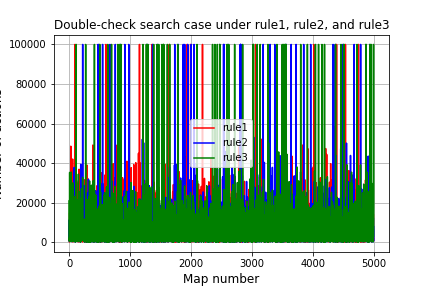
\includegraphics[width=0.7\textwidth]{fig/part1-q345.png}
		\caption{Number of actions in double-check search case}
		\label{fig:part1-q345.png}
	\end{figure}
	
	
	From the figure above, we can see that the performance of Rule 1 is the worst. Rule 2
	and Rule 3 are similar. The means of Rule1, Rule 2, and Rule 3 are 6287.49, 5223.53,
	and 5145.19. The average number of actions of Rule 3 is the smallest one among three
	rules. So, Rule 3 is the best. The variances of Rule1, Rule 2, and Rule 3 are
	54138591.92, 42819190.19, and 39314588.23. From this view, we can also conclude
	that Rule 3 is better. When the number of search actions is beyond 100000, we call it
	unsolvable because it is extremely hard to find the target under this circumstance. The
	fail rate of Rule1, Rule 2, and Rule 3 are 0.0026, 0.008, 0.0116. Rule 3 may sometimes
	not be able to find the target although it performs better.
	
	\item {Consider modifying the problem in the following way: at any time, you may only search the cell at your
		current location, or move to a neighboring cell (up/down, left/right). Search or motion each constitute a single
		`action'. In this case, the `best' cell to search by the previous rules may be out of reach, and require travel.
		One possibility is to simply move to the cell indicated by the previous rules and search it, but this may incur a
		large cost in terms of required travel. How can you use the belief state and your current location to determine
		whether to search or move (and where to move), and minimize the total number of actions required? Derive a
		decision rule based on the current belief state and current location, and compare its performance to the rule
		of simply always traveling to the next cell indicated by \textbf{Rule 1} or \textbf{Rule 2}. Discuss.} \\
	
	In this question, we need to move to the cell that we want to search and motion also
	counted as one step. We call this “search and motion case”. We use 3 rules to guide our
	search. Rule 1 means just traveling to the “best” cell which is indicated by the original
	Rule 1. Rule 2 is the same case. Rule 4 is invented by ourselves. It uses new criterion to
	supervise our search. We generate 5000 maps and use different rules to search the
	target in the maps. The result is shown in Fig \ref{fig:q4}.
	
	\begin{figure}[H]
		\centering
		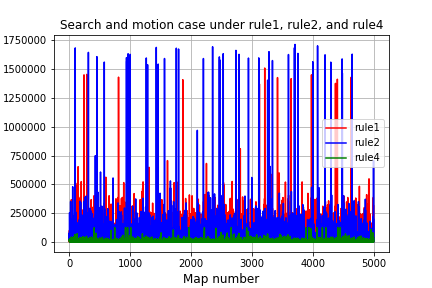
\includegraphics[width=0.7\textwidth]{fig/part1-q4.png}
		\caption{Number of actions in search and motion case}
		\label{fig:q4}
	\end{figure}
	
	From the figure, we can see that the performance of Rule 4 is better than Rule 1 and
	Rule 2. The means of Rule1, Rule 2, and Rule 4 are 58475.71, 45925.69, and 9745.66. It
	is easy to find that the average number of actions of Rule 4 is much smaller than Rule 1
	and Rule 2. The variances of Rule1, Rule 2, and Rule 4 are 7920337425.95,
	5069004957.26, and 119653468.99. From this view, we can also conclude that Rule 4 is
	better. When the number of search actions is beyond 100000, we call it unsolvable
	because it is extremely hard to find the target under this circumstance. The fail rate of
	Rule1, Rule 2, and Rule 4 are 0.0026, 0.0076, and 0.003. Rule 4 also performs well.
	
	
	\item {An old joke goes something like the following: 
		\begin{center}
			\textit{A policeman sees a drunk man searching for something under a streetlight and asks what the drunk has lost.
				He says he lost his keys and they both look under the streetlight together. After a few minutes the policeman
				asks if he is sure he lost them here, and the drunk replies, no, and that he lost them in the park. The
				policeman asks why he is searching here, and the drunk replies, ”the light is better here”.}
		\end{center}
		\par{In light of the results of this project, discuss.}
		}
\end{enumerate}

\section{A Moving Target}
\label{sec:A Moving Target}
\par{In this section, the target is no longer stationary, and can move between neighboring cells. Each time you perform
	a search, if you fail to find the target the target will move to a neighboring cell (with uniform probability for each).
	However, all is not lost - whenever the target moves, surveillance reports to you that the target was seen at a \textbf{Type1
	$ \times $ Type2} border where Type1 and Type2 are the cell types the target is moving between (though it is not reported
	which one was the exit point and which one the entry point. }
	
\par{Implement this functionality in your code. How can you update your search to make use of this extra information?
	How does your belief state change with these additional observations? Update your search accordingly, and again
	compare \textbf{Rule 1} and \textbf{Rule 2}.}

\par{Re-do question 4) above in this new environment with the moving target and extra information.}
\begin{enumerate}
	\item {Update search results} \\
	For a given block, there are 2 different search results: `True'(find the target) and `False'(Target not found). If the result is `True', this board is done. If the result is `False', we have to update the `prob' to represent this result.
		
	Using the notion of particle filter, assuming that each block have $p_i$ samples. If we have not found a target in $block_k$, some samples should be cast off, i.e. $p_k' = p_k(1-q_k)$. Then, resample all blocks by multiplying $\alpha$, where $\alpha = \frac{1}{1-p_kq_k}$
		
	In a nutshell, after searching $block_k$: 
	$p_i' = \alpha p_i$, where $i\ne k$; 
	$p_k' = \alpha p_k(1-q_k)$
	$\alpha = \frac{1}{1-p_kq_k}$
	
	The pseudo code is as follows:
	\begin{algorithm}[H]
		\caption{updateP(pos)}
		\begin{algorithmic}
			\STATE prob[pos] = prob[pos] * failP[cell[pos]]
			\STATE normalize(prob)
			\RETURN 
		\end{algorithmic}
	\end{algorithm}
	\begin{algorithm}[H]
	\caption{normalize(prob)}
	\begin{algorithmic}
		\STATE normalize(prob):
		\STATE sumP = sum(prob)
		\STATE prob = prob / sumP
		\RETURN 
	\end{algorithmic}
	\end{algorithm}

	In this problem, the target is moving and we can search the cell that we are interested in
	directly. We don’t need to move to the cell that we decide to search. We call this case
	“Moving case”. We use Rule 1, Rule 2, and Rule 5 to supervise our search. Rule 1 and
	Rule 2 are the same as we mentioned before. Rule 5 is designed by ourselves. 5000
	maps are generated and searched under 3 rules. The result is shown in Fig \ref{fig:part2-first}.
	
	\begin{figure}[H]
		\centering
		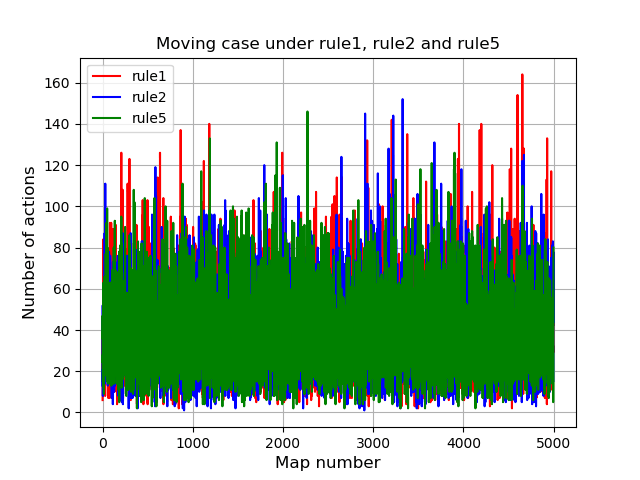
\includegraphics[width=0.7\textwidth]{fig/part2-first.png}
		\caption{Number of actions in moving case}
		\label{fig:part2-first}
	\end{figure}
	
	From the figure above, we find that the performance of 3 rules are similar to each other.
	The means of Rule1, Rule 2, and Rule 5 are 39.25, 37.82, and 38.04, which is close to
	
	each other. The variances of Rule1, Rule 2, and Rule 5 are 379.82, 347.52, and 351.06,
	which is also similar.
	
	\item {Update with additional observations} \\
	Using the notion of particle filter, we can update reports easily. For a given cell, if it is not a possible previous block, all its samples should be ruled out. If it is a possible previous block, and if there are some possible neighbors according to the reports, its samples will migrate to them. But if there are no possible neighbors, all its samples will also be trapped in this block and die out. Then, resample all blocks.
	
	Yet, notice that reports are related to each other. For example, 2 consecutive reports H-F, C-H tell far more than “the target first move from Hilly to Flat or from Flat to Hilly, and then move form Cave to Hilly or from Hilly to Cave”. We know that the target must move from Flat to Hilly and then to Cave.
	
	Therefore, we should consider each consecutive pair of reports and try to figure out the real moving direction. Once we know the real direction, we can pin down the direction of future reports, but also all previous reports.
	
	Notice that if we know the real direction of previous reports, we should re-filter all previous observations because observations have become more accurate.
	
	The pseudo code is as follows:
	\begin{algorithm}[H]
		\caption{updateR(report)}
		\begin{algorithmic}
			\STATE{reUpFlag, directions = solveReprot(report)}
			\IF{reUpFlag}
				\STATE{reUpdateReport(searchHistory, targetHistory)}
			\ELSE
				\STATE{updateReport(directions)}
			\ENDIF
			\RETURN
		\end{algorithmic}
	\end{algorithm}
	\begin{algorithm}[H]
		\caption{solveReport(report)}
		\begin{algorithmic}
			\IF{reportSolved}
				\STATE {direction = trackTarget(report, targetHistory[-1])}
				\STATE reUpFlag = False
			\ELSE
				\STATE {common = findCommon(report, reportHistory[-1])}
				\IF{len(common) == 1} 
					\STATE{backtrack(common, reportHistory)}
					\STATE{direction = tarckTarget(report, targetHistory[-1])}
					\STATE{reUpFlag = True}
				\ELSE
					\STATE{direction = (report, report.reverse())}
					\STATE{reUpFlag = False}
				\ENDIF
			\ENDIF
			\STATE reportHistory.append(report)
			\RETURN reUpFlag, direction
		\end{algorithmic}
	\end{algorithm}
	\begin{algorithm}[H]
		\caption{reUpdateReprot(searchHistory, targetHistory)}
		\begin{algorithmic}
			\FOR{i in range(searchHistory)}
				\STATE updateP(searchHistory[i])
				\STATE updateReport(((targetHistory[i], targetHistory[i+1]), ))
			\ENDFOR
			\RETURN 
		\end{algorithmic}
	\end{algorithm}
	\begin{algorithm}[H]
		\caption{updateReprot(directions)}
		\begin{algorithmic}
			\STATE{tempProb = zeros\_like(prob)}
			\FOR{prev, post in directions}
				\FOR{each block pos}
					\IF{cell[pos] == prev}
						\STATE{nPosList = where(border[pos, post])}
						\STATE{factor = len(nPosList)}
						\IF{factor}
							\FOR{each nPos in nPosList}
								\STATE{tempPorb[nPos] = tempPorb[nPos] + prob[pos] / factor}
							\ENDFOR
						\ENDIF
					\ENDIF
				\ENDFOR
			\ENDFOR
			\STATE{prob = normalize(tempProb)}
			\RETURN 
		\end{algorithmic}
	\end{algorithm}
	\begin{algorithm}[H]
		\caption{trackTarget(report, prev)}
		\begin{algorithmic}
			\STATE post = report - prev
			\STATE targetHistory.append(post)
			\RETURN post
		\end{algorithmic}
	\end{algorithm}
	\begin{algorithm}[H]
		\caption{backtrack(post, reportHistory)}
		\begin{algorithmic}
			\STATE targetHisory.insert(0, post)
			\FOR{report in reportHistory.reverse()}
				\STATE prev = reprot - post
				\STATE targetHistory.insert(0, prev)
			\ENDFOR
			\RETURN 
		\end{algorithmic}
	\end{algorithm}

	In this problem, the target is moving and motion also counted as one step. We call this
	case “moving and motion”. We use three rules to guide our search --- Rule 1, Rule 2, and
	Rule 5. Rule 1 and Rule 2 are just the original rules where motion is one step now. Rule 5
	is designed for this specific problem. We generate 5000 maps and use these 3 rules to
	search the target in the maps. The result is shown in Fig \ref{fig:part2-last.png}.
	
	
	\begin{figure}[H]
		\centering
		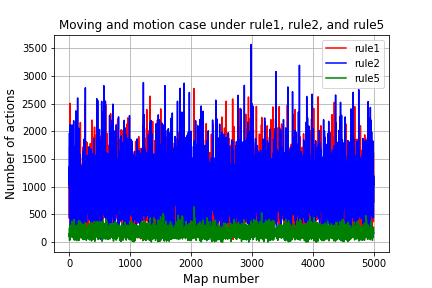
\includegraphics[width=0.7\textwidth]{fig/part2-last.png}
		\caption{Number of actions in moving and motion case}
		\label{fig:part2-last.png}
	\end{figure}
	
	From the figure above, it is easy to find that the performance of Rule 5 is better than Rule
	1 and Rule 2. The means of Rule1, Rule 2, and Rule 5 are 938.88, 991.54, and 177.54.
	We can see that the average number of actions of Rule 5 is smaller than Rule 1 and Rule
	2. The variances of Rule1, Rule 2, and Rule 5 are 154395.57, 176673.58, and 5534.82.
	From this view, we can also conclude that Rule 5 is better.
	
\end{enumerate}
\end{document}